\chapter{Data Understanding}

The dataset is composed by 10000 records. Each record represents a customer, described by $24$ different attributes.

\medskip

\section{Data semantics, distribution and statistics}

In this section we will analyze, for each attribute, its semantic and we will show interesting statistic and plot.
We have used two different colors for who went in credit default (green) and not (red) in order to better visualize their distribution among the different attributes.

We have discretized the continuous attributes by using the natural binning method. 

For these attributes the mode of the bin has also been reported as it is more representative.

%%%%%%%%%%%%%%%%%%%%%%%%%%%%%%%%%%%%%%%%%%%%%%%%%%%%%%
\smallskip
\begin{figure}[h]
  \begin{minipage}[h]{.50\textwidth}
        {\Large \textbf{Sex}}
        
        Gender of the customer.
        
        A binary attribute that can assume the values of \textit{male} ($3868$ of $10000$) or \textit{female} ($6032$ of $10000$). 
        
        Both of the gender values have a similar credit default rate ($25\%$ for males and $20\%$ for females).
  \end{minipage}
  \begin{minipage}[h]{.50\textwidth}
    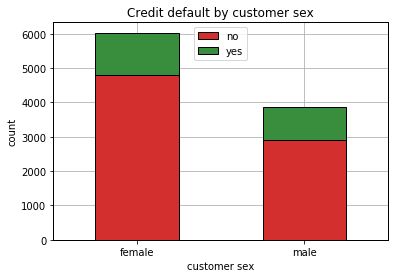
\includegraphics[width=.95\textwidth]{img/ch2/sex}
  \end{minipage}
\end{figure}

%%%%%%%%%%%%%%%%%%%%%%%%%%%%%%%%%%%%%%%%%%%%%%%%%%%%%%
\begin{figure}[h]
  \begin{minipage}[h]{.45\textwidth}
    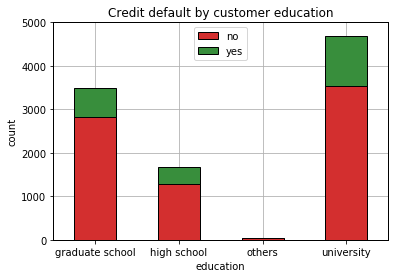
\includegraphics[width=.95\textwidth]{img/ch2/education}
  \end{minipage}
  \begin{minipage}[h]{.50\textwidth}
        {\Large \textbf{Education}}
        
        Qualification of the customer.
        
        A categorical attribute that can assume the values of 
        \textit{university} ($4685$ of $10000$),
        \textit{high school} ($1672$ of $10000$),
        \textit{graduate school} ($3480$ of $10000$) or
        \textit{others} ($36$ of $10000$).
        The default rate is again very similar for all the qualifications (around the $20\%$), except for the \textit{others} which is equal to $5\%$, but its number of records is very low to make any assumptions.
  \end{minipage}
\end{figure}

%%%%%%%%%%%%%%%%%%%%%%%%%%%%%%%%%%%%%%%%%%%%%%%%%%%%%%
\smallskip
\begin{figure}[h]
  \begin{minipage}[h]{.50\textwidth}
        {\Large \textbf{Status}}
        
        Marital status of the customer.
        
        A categorical attribute that can assume the values of 
        \textit{married} ($4685$ of $10000$),
        \textit{single} ($3757$ of $10000$) or
        \textit{other status} ($75$ of $10000$).
        
        The default rate is very similar for all the status (around the $25\%$).
  \end{minipage}
  \begin{minipage}[h]{.45\textwidth}
    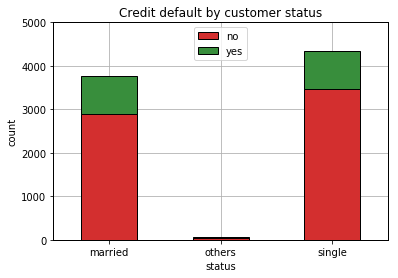
\includegraphics[width=.95\textwidth]{img/ch2/status}
  \end{minipage}
\end{figure}

%%%%%%%%%%%%%%%%%%%%%%%%%%%%%%%%%%%%%%%%%%%%%%%%%%%%%%
\smallskip
\begin{figure}[h]
  \begin{minipage}[h]{.45\textwidth}
    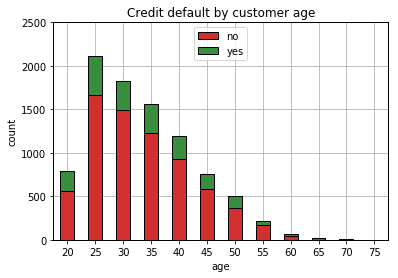
\includegraphics[width=.95\textwidth]{img/ch2/age}
  \end{minipage}
  \begin{minipage}[h]{.50\textwidth}
        {\Large \textbf{Age}}
        
        Age of the customer.
        
        An attribute that in the dataset assume integer values in $[21, 75]$, the lower limit to $21$ is due that in Taiwan the age of majority is $20$, on the other hand the upper limit can be as high as humanly possible.
        
        The average age is $35.49$, the standard deviation is $9.22$.
        The mode is $29$ and the median is $34$.
        The $50\%$ of the ages lie in $[28, 41]$.
        
        We decide to set a bin to $5$ year as it represent a good trade-off between the size and number of bins. The bin with most elements is $25$.
        
        Again the default rate is similar for all the bins (around $25\%$).
  \end{minipage}
\end{figure}

%%%%%%%%%%%%%%%%%%%%%%%%%%%%%%%%%%%%%%%%%%%%%%%%%%%%%%
\smallskip

\begin{figure}[h]
  \begin{minipage}[h]{.50\textwidth}
        {\Large \textbf{Limit}}
        
        Limit of the credit card (expressed in NT dollar).
        
        It is the maximum amount the credit card company will let borrow on the account, 
        a continuous attribute that can assume values in $[10000, 780000]$ (all values are multiples of $10000$).
        
        The average is $167197$ and the standard deviation is $128975$, $50\%$ of the ages lie in $[50000, 240000]$. The bin with most elements is $50000$.
        
        The default rate in this case is very different for each bin as it decrease with the limit: the first bin has a default rate of $38\%$, the second one of $26\%$ and around $10\%$ for the last bin.
        
  \end{minipage}
  \begin{minipage}[h]{.45\textwidth}
    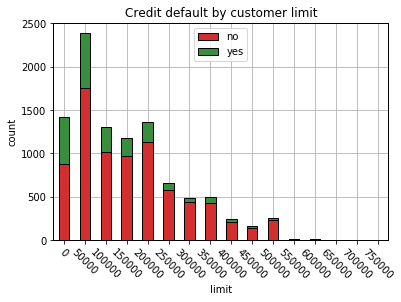
\includegraphics[width=.95\textwidth]{img/ch2/limit}
  \end{minipage}

\end{figure}

%%%%%%%%%%%%%%%%%%%%%%%%%%%%%%%%%%%%%%%%%%%%%%%%%%%%%%

\smallskip
\begin{figure}[h]
  \begin{minipage}[h]{.50\textwidth}
    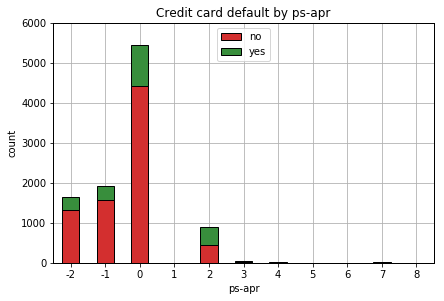
\includegraphics[width=.95\textwidth]{img/ch2/payment_status_1}
  \end{minipage}
  \begin{minipage}[h]{.50\textwidth}
        {\Large \textbf{Payment status}}
        
        History of past payments.
        
        Six categorical attributes that represent the repayment status, one for each month between April and September.
        A payment status is an integer number in the range $[-2, 9]$ where:
        
         $-2$ = no consumption
         
         $-1$ = paid in full
         
         $0$ = the use of revolving credit

         $1$ = payment delay for one month

         $2$ = payment delay for two months
         
         ...
         
         The distribution of the payment status over the six months are all very similar to each other so we only illustate the first one for simplicity.
         The most frequent bin is always the $0$ and around $90\%$ of the customers always lies between $-2$ and $0$. 

  \end{minipage}
\end{figure}



%%%%%%%%%%%%%%%%%%%%%%%%%%%%%%%%%%%%%%%%%%%%%%%%%%%%%%
\smallskip
\begin{figure}[h]
  \begin{minipage}[h]{.50\textwidth}
        {\Large \textbf{Bill Amount}}
        
        Amount of bill statement (expressed in NT dollar).
        
        Six continuous attributes, again one for each month between April and September.
        The values are in range
        
  \end{minipage}
  \begin{minipage}[h]{.50\textwidth}
    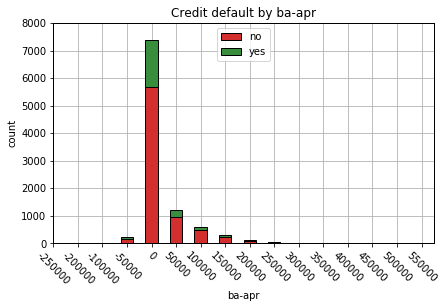
\includegraphics[width=.95\textwidth]{img/ch2/bill_amount_1}
  \end{minipage}
\end{figure}

%%%%%%%%%%%%%%%%%%%%%%%%%%%%%%%%%%%%%%%%%%%%%%%%%%%%%%
\smallskip
\begin{figure}[h]
  \begin{minipage}[h]{.50\textwidth}
    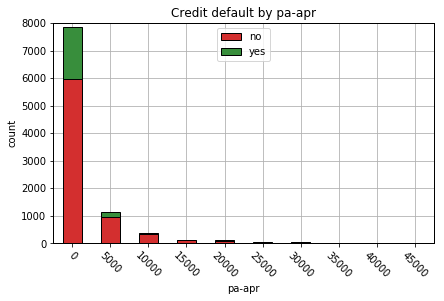
\includegraphics[width=.95\textwidth]{img/ch2/payment_amount_1}
  \end{minipage}
  \begin{minipage}[h]{.50\textwidth}
        {\Large \textbf{Payment amount}}
  \end{minipage}
\end{figure}
%%%%%%%%%%%%%%%%%%%%%%%%%%%%%%%%%%%%%%%%%%%%%%%%%%%%%%
\smallskip
\begin{figure}[ht]
  \begin{minipage}[h]{.60\textwidth}
        {\Large \textbf{Credit default}}
        
        prova
  \end{minipage}
  \begin{minipage}[h]{.40\textwidth}
    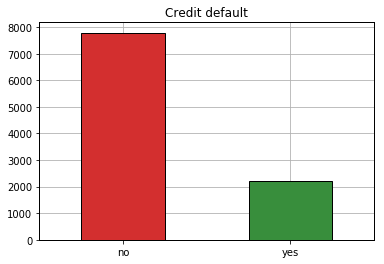
\includegraphics[width=.95\textwidth]{img/ch2/credit_default}
  \end{minipage}
\end{figure}

%%%%%%%%%%%%%%%%%%%%%%%%%%%%%%%%%%%%%%%%%%%%%%%%%%%%%%%%%%%%%%%%%%%%%%%%%%%%%%%
\clearpage

\section{Assessing data quality}

\begin{figure}[h]
  \begin{minipage}[h]{.60\textwidth}

    In this part we have checked for duplicates and outliers, in order to reduce the quantity of data and to avoid that their presence could negatively affect
  \end{minipage}
  \begin{minipage}[h]{.40\textwidth}
    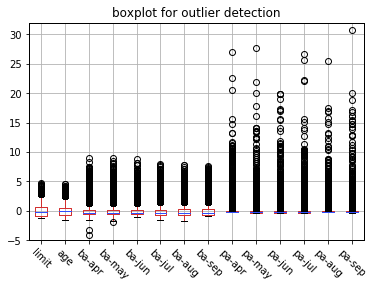
\includegraphics[width=.95\textwidth]{img/ch2/outlier}
  \end{minipage}
\end{figure}

%%%%%%%%%%%%%%%%%%%%%%%%%%%%%%%%%%%%%%%%%%%%%%%%%%%%%%%%%%%%%%%%%%%%%%%%%%%%%%%
\section{Variables transformations}

modifica variabili

modifica variabili

modifica variabili


%%%%%%%%%%%%%%%%%%%%%%%%%%%%%%%%%%%%%%%%%%%%%%%%%%%%%%%%%%%%%%%%%%%%%%%%%%%%%%%

\section{Correlations and redundant variables}

\begin{figure}[h]
  \begin{minipage}[h]{.60\textwidth}
  Analyzing the correlation matrix of all the continuous attribute we can clearly see that all the attributes related to the bill amount are strongly correlated.
  All the 
  
  \end{minipage}
  \begin{minipage}[h]{.40\textwidth}
    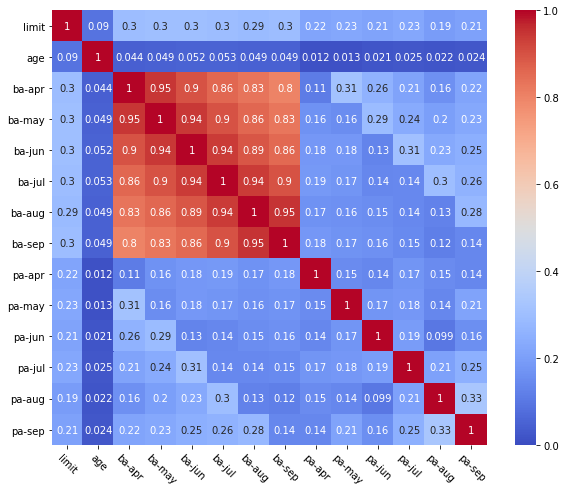
\includegraphics[width=.95\textwidth]{notebook/CardCardDefault_84_1}
  \end{minipage}
\end{figure}


\begin{figure}[h]
  \begin{minipage}[h]{.40\textwidth}
    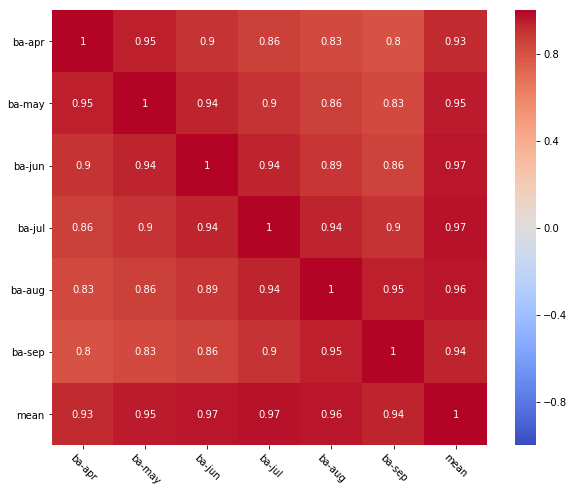
\includegraphics[width=.95\textwidth]{notebook/CardCardDefault_86_1}
  \end{minipage}
  \begin{minipage}[h]{.60\textwidth}
  We add a new attribute to the dataset called \textit{ba\_mean} which is the mean of all the bill amount for each customer.
  We plot now a new correlation matrix rescricted only to the attributed of.
  \end{minipage}
\end{figure}
